\documentclass{beamer}
\usetheme{Warsaw}

\usepackage[utf8]{inputenc}
\usepackage{fancybox}
\usepackage{multimedia} 
\usepackage{subfig}
\usepackage{amsmath}
\usepackage{hyperref}
\usepackage[all]{xy}
\begin{document}


\title[Angewandte Mathematik] % (optional, only for long titles)
{Angewandte Mathematik
\\

\includegraphics[scale=0.15]{images/cover}
}
\subtitle{}
\author[Dr. Johannes Riesterer] % (optional, for multiple authors)
{Dr.  rer. nat. Johannes Riesterer}

\date[KPT 2004] % (optional)
{}

\subject{Angewandte Mathematik}



\frame{\titlepage}

\begin{frame}
    \frametitle{Angewandte Mathematik}
    \begin{block}{Wiederholung Taylorreihe für 1-dimensionale Funktionen}
        Für eine $\mathcal{C}^{n}$-Funktion $f: \mathbb{R} \to \mathbb{R}$ und $a \in \mathbb{R}$ ist die Taylorreihe um $a$ gegeben durch
    \begin{align*}
        T_N f(x;a) := \sum_{n=0}^N \frac{f^{(n)}(a)}{n!} (x-a)^n
    \end{align*}
    \href{https://de.wikipedia.org/wiki/Taylorreihe}{Taylorreihe Wiki}
    \end{block}

    \begin{block}{Wiederholung Taylorreihe für 1-dimensionale Funktionen}
        Für eine $\mathcal{C}^{n+1}$-Funktion $f: \mathbb{R} \to \mathbb{R}$ und $a \in \mathbb{R}$ gilt
    \begin{align*}
        f(x) = T_n f(x; a) + R_n f(x; a) = T_n f(x; a) + o(|x - a|^n), \quad x\rightarrow a
    \end{align*}
    \href{https://de.wikipedia.org/wiki/Taylor-Formel}{Taylorreihe Wiki}
    \end{block}
\end{frame}




\begin{frame}
    \frametitle{Angewandte Mathematik}


    \begin{block}{Wiederholung Taylorreihe für 1-dimensionale Funktionen}
        Wie kann man das auf höhere Dimensionen verallgemeinern und was für Eigenschaften brauchen wir dafür?
        \end{block}
\end{frame}


\begin{frame}
    \frametitle{Angewandte Mathematik}
\framesubtitle{Vertauschen von Ableitungen}
    \begin{block}{Satz von Schwarz}
Wenn Für eine Funktion $f:  U \subset \mathbb{R}^n \to \mathbb{R}$ die Ableitungen $\frac{\partial}{\partial x_i} f(a)$, $\frac{\partial}{\partial x_j}f(a)$ und $ \frac{\partial}{\partial x_i}\frac{\partial }{\partial x_j} f(a)$ existieren und letztere stetig ist, dann existiert auch $ \frac{\partial}{\partial x_j}\frac{\partial }{\partial x_i} f(a)$ und es gilt
\begin{align*}
\frac{\partial}{\partial x_i}\frac{\partial }{\partial x_j} f(a) = \frac{\partial}{\partial x_j}\frac{\partial }{\partial x_i} f(a)
\end{align*}
\end{block}
    \begin{block}{Bedeutung}
Die Reihenfolge spielt beim wiederholten ableiten keine Rolle.
\end{block}
 \end{frame}



\begin{frame}
    \frametitle{Angewandte Mathematik}
\framesubtitle{Höhere Ableitungen}
    \begin{block}{$\mathcal{C}^k$-Funktionen}
Eine  Funktion  $f: U \subset \mathbb{R}^n \to \mathbb{R}$ für die alle partiellen Ableitungen 
\begin{align*}
 \frac{\partial}{\partial x_{i_1}} \cdots   \frac{\partial}{\partial x_{i_k}} f(a)
\end{align*}
mit $i_1 + \cdots + i_k \leq k$ existieren und stetig sind heißt $\mathcal{C}^k$-Funktion oder $k$-mal stetig differenzierbar.
\end{block}
%    \begin{block}{$\mathcal{C}^k$-Funktionen}
% Eine  $\mathcal{C}^1$-Funktion ist also eine differenzierbare Funktion.
%\end{block}
 \end{frame}


\begin{frame}
    \frametitle{Angewandte Mathematik}
\framesubtitle{Höhere Ableitungen}
    \begin{block}{p-te Ableitung}
Für  eine Funktion  $f: U \to \mathbb{R}$, $a \in U$ und Vektoren $v^1, \cdots , v^p \in \mathbb{R}^n$ heißt 
\begin{align*}
d^pf(a) \bigl(v^1, \cdots , v^p  ) := \partial_{v^1} \hdots \partial_{v^p} f(a)
\end{align*}
die $p$-te Richtungsableitung von $f$. Sie ist wegen dem Satz von Schwarz wohldefiniert.

\end{block}
    \begin{block}{}
\begin{align*}
d^pf(a) \bigl(v^1, \cdots , v^p  ) = \sum_{i_1 = 1}^n \cdots \sum_{i_p = 1}^n  \frac{\partial}{\partial x_{i_1}} \hdots \frac{\partial}{\partial x_{i_p}} f(a) \cdot v^1_{i_1} \cdots v^p_{i_p} \; .
\end{align*}
Für einen Vektor $z \in \mathbb{R}^n$ definieren wir $d^pf(a) z^p := d^pf(a) \underbrace{(z, \cdots , z)}_{p-mal} \;.$

\end{block}
 \end{frame}


\begin{frame}
    \frametitle{Angewandte Mathematik}
\framesubtitle{Höhere Ableitungen}
    \begin{block}{Hessematrix}
Für $p = 2$ und $u,v \in \mathbb{R}^n$ ist
\begin{align*}
d^2f(a) \bigl(u , v ) = \sum_{i = 1}^n \sum_{j = 1}^n \frac{\partial}{\partial x_{i}}  \frac{\partial}{\partial x_{j}} f(a) v_{i}  u_{i} 
\end{align*}
und mit 
\begin{align*}
f''(a) : = \begin{pmatrix}  \frac{\partial}{\partial x_{1}} \frac{\partial}{\partial x_{1}} f(a)   &  \cdots &  \frac{\partial}{\partial x_{1}} \frac{\partial}{\partial x_{n}} f(a) \\
\vdots & & \vdots  \\
 \frac{\partial}{\partial x_{n}} \frac{\partial}{\partial x_{1}} f(a)   &  \cdots &  \frac{\partial}{\partial x_{n}} \frac{\partial}{\partial x_{n}} f(a)
\end{pmatrix} 
\end{align*}
ist $d^2f(a) \bigl(u , v ) = u^T  \cdot f''(a) \cdot v$. Die Matrix $f''(a)$ wird auch Hesse-Matrix genannt. Nach dem Satz von Schwarz ist sie symmetrisch.
\end{block}
 \end{frame}

\begin{frame}
    \frametitle{Angewandte Mathematik}
\framesubtitle{Höhere Ableitungen}
    \begin{block}{Taylorapproximation}
Sei   $f:  U \subset \mathbb{R}^n \to \mathbb{R}$ eine $\mathcal{C}^{p+1}$-Funktion und $x,a \in U$, so dass die Verbindung zwischen $x$ und $a$ in $U$ liegt.
Dann gilt
\begin{align*}
f(x) = f(a) + \sum_{k=1}^{p}\frac{1}{p!} d^k f(a) (x-a)^k + R_{p+1} (x;a)
\end{align*}
mit dem Restglied $R_{p+1} (x;a) =   o(||x - a||^n)$.

\end{block}
 \end{frame}


\begin{frame}
    \frametitle{Angewandte Mathematik}
\framesubtitle{Höhere Ableitungen}
    \begin{block}{Beweis}
Sei $F(t) := f(a + th)$ mit $t \in [0,1]$. Wiederholte Anwendung der Kettenregel mit $\gamma(t) := a +th$ ergibt
\begin{align*}
& F'(t) = \sum_{i=1}^n  \frac{\partial}{\partial x_{i}} f(a + th) h_i \\
& F''(t) =\sum_{j=1}^n \sum_{i=1}^n   \frac{\partial}{\partial x_{j}} \frac{\partial}{\partial x_{i}} f(a + th) h_i h_j \\
& \vdots \\
& F^p(t) =  \sum_{i_1=1}^n  \cdots \sum_{i_p=1}^n   \frac{\partial}{\partial x_{i_1}} \cdots \frac{\partial}{\partial x_{i_p}} f(a + th) h_{i_1} \cdots  h_{i_p}  \; .
\end{align*}
\end{block}
 \end{frame}

\begin{frame}
    \frametitle{Angewandte Mathematik}
\framesubtitle{Höhere Ableitungen}
    \begin{block}{Beweis}
Für $h := (x-a)$  ist $F(0) = f(a)$ und $F(1)= f(x)$ 
und mit der Taylorapproximation für Funktionen einer Veränderlichen  

\begin{align*}
 F(1) = F(0) + F'(0) + \frac{1}{2!} F''(0) + \cdots + \frac{1}{p!} F^p(0) + R_{p+1} 
\end{align*}
\end{block}
 \end{frame}



\begin{frame}
    \frametitle{Angewandte Mathematik}
\framesubtitle{Extrema}
    \begin{block}{Extrema}
 Ist $f: U  \to \mathbb{R}$ eine $\mathcal{C}^2$-Funktion und ist $f'(a) = 0$ für ein $a \in U$. Dann gilt:
\begin{itemize}
\item $f''(a) > 0 \Rightarrow $ $f$ hat in $a$ ein isoliertes lokales Minimum.
\item $f''(a) < 0 \Rightarrow $ $f$ hat in $a$ ein isoliertes lokales Maximum.
\item $f''(a) \gtrless 0 \Rightarrow $ $f$ hat in $a$ einen Sattelpunkt.
\end{itemize} 
\end{block}

\begin{block}{Positive/negative Definitheit}
   \begin{itemize}
   \item $f''(a) > 0 \Leftrightarrow \forall h \in \mathbb{R}^n \; h^t f''(a) h > 0$.
   \item $f''(a) < 0 \Leftrightarrow \forall h \in \mathbb{R}^n \; h^t f''(a) h < 0$.
   \item $f''(a) \gtrless 0 \Leftrightarrow h^t f''(a) h \gtrless 0$.
   \end{itemize} 
   \end{block}

 \end{frame}

 \begin{frame}
    \frametitle{Angewandte Mathematik}
\framesubtitle{Extrema}
 \begin{figure}[H]
    \centering
  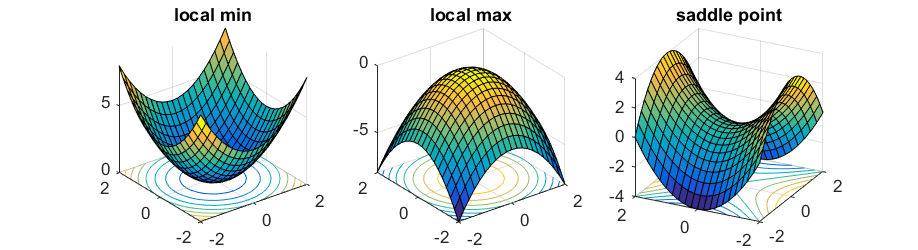
\includegraphics[width=1.0\textwidth]{images/minmaxsaddle.png}
\end{figure}
\end{frame}

\begin{frame}
    \frametitle{Angewandte Mathematik}
\framesubtitle{Extrema}
    \begin{block}{Beweis}

Sei $f'(a) = 0$ und $f''(a) > 0$. Mit der Taylorformel gilt für hinreichend kurze Vektoren $h \in \mathbb{R}^n$
\begin{align*}
f(a + h) = f(a) + \frac{1}{2} h^T f''(a) h + R(h)
\end{align*}
mit $\lim_{h \to 0} \frac{R(h)}{ ||h||^2} = 0$. 
Die Funktion $v^T f''(a) v $ hat ein positives Minimum  $m$ auf der Einheitssphäre $\{ v \in \mathbb{R}^n \; | \; ||v|| = 1 \}$ da $f''(a) > 0$.
Damit erhalten wir die Abschätzung
\begin{align*}
 h^T f''(a) h  = ||h|| \frac{1}{||h||} h^t  f''(a)  ||h|| \frac{1}{||h||} h \geq m ||h||^2 \;.
\end{align*}
\end{block}
 \end{frame}



\begin{frame}
    \frametitle{Angewandte Mathematik}
\framesubtitle{Extrema}
    \begin{block}{Beweis}
Wir wählen $\epsilon$ so klein, dass $R(h) \leq \frac{m}{2}  ||h||^2$ gilt für $||h|| < \epsilon$  (was geht wegen Taylorformel).
Damit erhalten wir
\begin{align*}
f(a + h) \geq f(a) +  m ||h||^2 \;.
\end{align*}
und damit hat $f$ ein lokales Minimum in $a$.

Der Fall $f''(a) < 0$ wird mit Betrachtung von $-f$ durch den vorigen Fall bewiesen.
\end{block}
 \end{frame}



\begin{frame}
    \frametitle{Angewandte Mathematik}
\framesubtitle{Extrema}
    \begin{block}{Beweis}


Es sei nun $f''(a) \gtrless 0$ und $v$ mit $v^T f''(a) v > 0$ und $w$ mit $w^T f''(a) w > 0$. Betrachten wir die Funktionen
\begin{align*}
F_v (t) := f(a + tv) \\
F_w(t) := f(a +tw)
\end{align*}
dann ist 
\begin{align*}
F_v' (t) = 0; \; F_v''(0) = v^T f''(a) v > 0 \\
F_w' (t) = 0; \; F_w''(0) = w^T f''(a) w < 0 \\
\end{align*}
und somit hat $F_v$ ein isoliertes lokales Maximum und $F_w$ ein isoliertes lokales Minimum und damit $f$ kein lokales Extremum  in  $a$.
\end{block}
 \end{frame}




 
 \begin{frame}
    \frametitle{Angewandte Mathematik}
    \framesubtitle{Positive Definitheit}
     \begin{itemize}
         \item Sei \( A \in \mathbb{R}^{n \times n} \) eine symmetrische Matrix.
         \item Behauptung: \( A \) ist genau dann positiv definit, wenn alle Eigenwerte von \( A \) positiv sind.
         \item Wir beweisen die beiden Richtungen:
         \begin{itemize}
             \item Positive Definitheit \( \Rightarrow \) Positive Eigenwerte
             \item Positive Eigenwerte \( \Rightarrow \) Positive Definitheit
         \end{itemize}
     \end{itemize}
 \end{frame}
 
 \begin{frame}{Richtung 1: Positive Definitheit \( \Rightarrow \) Positive Eigenwerte}
     \begin{itemize}
         \item Angenommen, \( A \) ist positiv definit. Das bedeutet:
         \[
         h^\top A h > 0 \quad \text{für alle } h \in \mathbb{R}^n \setminus \{0\}.
         \]
         \item Sei \( \lambda \) ein Eigenwert von \( A \) mit zugehörigem Eigenvektor \( v \neq 0 \), sodass \( A v = \lambda v \).
         \item Setze \( h = v \) und erhalte:
         \[
         v^\top A v = v^\top (\lambda v) = \lambda v^\top v.
         \]
         \item Da \( v^\top v > 0 \), folgt \( \lambda > 0 \).
   
         \item Da dies für jeden Eigenwert von \( A \) gilt, sind alle Eigenwerte von \( A \) positiv.
     \end{itemize}
 \end{frame}
 
 \begin{frame}{Richtung 2: Positive Eigenwerte \( \Rightarrow \) Positive Definitheit}
     \begin{itemize}
         \item Angenommen, alle Eigenwerte von \( A \) sind positiv.
         \item Da \( A \) symmetrisch ist, können wir \( A \) diagonalisieren:
         \[
         A = Q \Lambda Q^\top,
         \]
         wobei \( \Lambda \) eine Diagonalmatrix mit positiven Diagonaleinträgen ist.
     \end{itemize}
 \end{frame}
 
 \begin{frame}
    \frametitle{Angewandte Mathematik}
    \framesubtitle{Positive Definitheit}
     \begin{itemize}
         \item Für \( h \in \mathbb{R}^n \setminus \{0\} \):
         \[
         h^\top A h = h^\top Q \Lambda Q^\top h = (Q^\top h)^\top \Lambda (Q^\top h).
         \]
         \item Setze \( y = Q^\top h \). Da \( Q \) orthogonal ist, gilt \( y \neq 0 \) wenn \( h \neq 0 \).
         \item Dann ist:
         \[
         h^\top A h = y^\top \Lambda y = \sum_{i=1}^n \lambda_i y_i^2.
         \]
     \end{itemize}
 \end{frame}
 
 \begin{frame}
    \frametitle{Angewandte Mathematik}
    \framesubtitle{Positive Definitheit}
     \begin{itemize}
         \item Da \( \lambda_i > 0 \) für alle \( i \) und \( y \neq 0 \), folgt \( \sum_{i=1}^n \lambda_i y_i^2 > 0 \).
         \item Somit ist \( h^\top A h > 0 \) für alle \( h \neq 0 \).
         \item Also ist \( A \) positiv definit.
     \end{itemize}
 \end{frame}
 
 

 \begin{frame}
    \frametitle{Aufgabe 2 (Extrema)}
    Gegeben ist die Funktion \( f(x, y) = 4x^2 + y^2 - 4x - 6y + 4 \).
    
    \begin{enumerate}
        \item Bestimme die partiellen Ableitungen 1. Ordnung der Funktion \( f(x, y) \) bezüglich \( x \) und \( y \).
        \item Finde die kritischen Punkte der Funktion, indem du die partiellen Ableitungen gleich Null setzt und das resultierende Gleichungssystem löst.
        \item Bestimme die partiellen Ableitungen 2. Ordnung und bilde die Hesse-Matrix an den kritischen Punkten.
        \item Untersuche die Art der Extrema (Maximum, Minimum oder Sattelpunkt) anhand der Hesse-Matrix und der Determinantenkriterien.
        \item Interpretiere die Ergebnisse im Kontext der Funktion. Beschreibe, was die gefundenen Extrema über die Funktion aussagen.
    \end{enumerate}
\end{frame}

\begin{frame}
    \frametitle{Lösung 1: Partielle Ableitungen 1. Ordnung}
    Die partiellen Ableitungen 1. Ordnung sind:
    \begin{align*}
        \frac{\partial f}{\partial x} &= 8x - 4, \\
        \frac{\partial f}{\partial y} &= 2y - 6.
    \end{align*}

    Die kritischen Punkte ergeben sich aus:
    \begin{align*}
        8x - 4 &= 0, \\
        2y - 6 &= 0.
    \end{align*}
    Daraus folgt \( x = \frac{1}{2} \) und \( y = 3 \).
\end{frame}

\begin{frame}
    \frametitle{Lösung 3: Partielle Ableitungen 2. Ordnung und Hesse-Matrix}
    Die zweiten partiellen Ableitungen und die Hesse-Matrix lauten:
    \begin{align*}
        \frac{\partial^2 f}{\partial x^2} &= 8, \\
        \frac{\partial^2 f}{\partial y^2} &= 2, \\
        \frac{\partial^2 f}{\partial x \partial y} &= 0.
    \end{align*}
    Die Hesse-Matrix ist somit:
    \[
    \begin{pmatrix}
        8 & 0 \\
        0 & 2
    \end{pmatrix}
    \]


    \frametitle{Lösung 5: Interpretation der Ergebnisse}
  Die Eigenwerte der Hessematrix sind $8$ und $2$ und damit positiv. Die Funktion hat also in $(\frac{1}{2}, 3)$ ein lokales Minimum. 
\end{frame}


\end{document}

